\section{RISMC Approach to PRA}
\label{sec:rismc}

The RISMC approach~\cite{RISMC} employs both deterministic and stochastic methods 
in a single analysis framework (see Figure~\ref{fig:RISMCoverview}). In the deterministic method 
set we include:
\begin{itemize}
  \item Modeling of the thermal-hydraulic behavior of the plant~\cite{BWR_SBO_Mandelli,BWRanalysis}
  \item Modeling of external events such as flooding~\cite{mandelliPSA2015}
  \item Modeling of the operators’ responses to the accident scenario~\cite{HRA_BoringReport2014}
\end{itemize}

\begin{figure}
    \centering
    \centerline{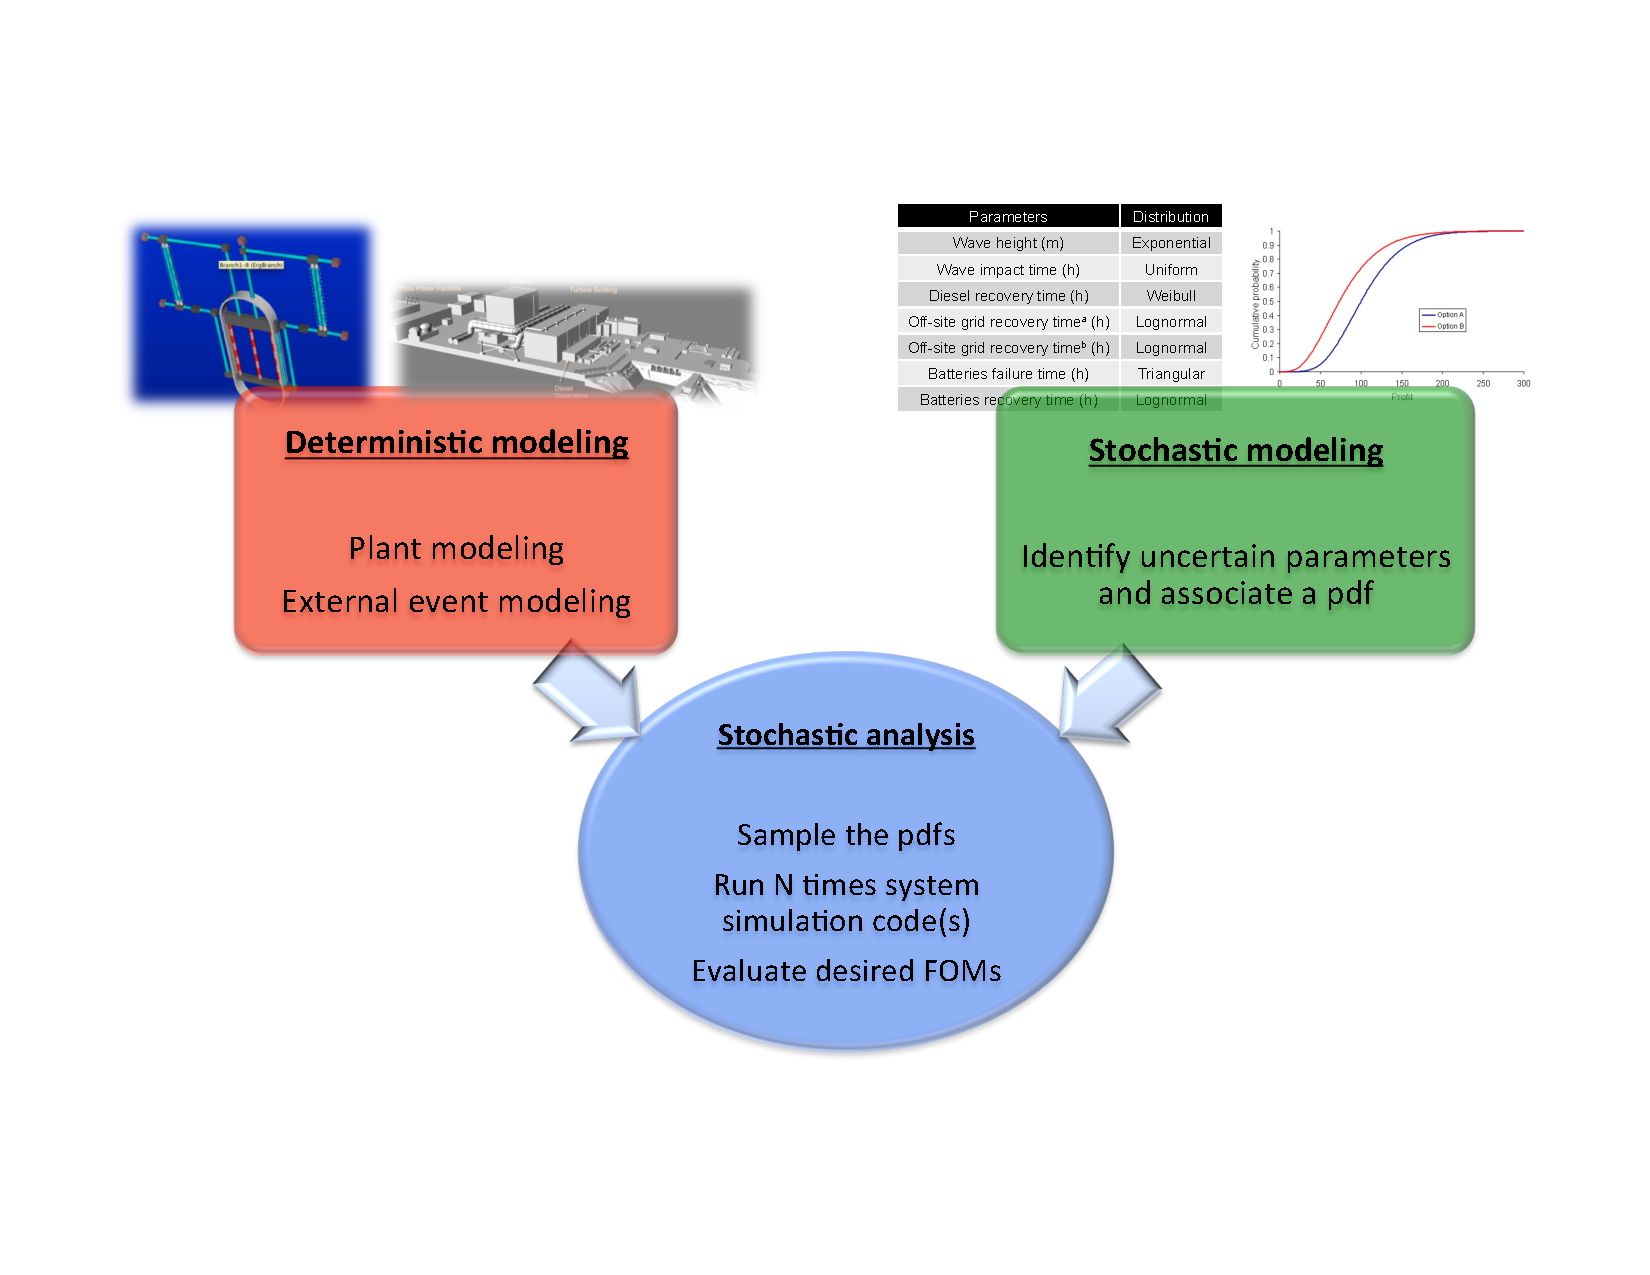
\includegraphics[scale=0.4]{RISMCoverview.pdf}}
    \caption{Overview of the RISMC approach}
    \label{fig:RISMCoverview}
\end{figure}

Note that deterministic modeling of the plant or external events can be performed by employing specific 
simulator codes but also surrogate models~\cite{ROM}, known as reduced order models (ROM). ROMs would 
be employed 
in order to decrease the high computational costs of employed codes. In addition, multi-fidelity codes 
can be employed to model the same system; the idea is to switch from low-fidelity to high-fidelity code 
when higher accuracy is needed (e.g., use low-fidelity codes for steady-state conditions and high-fidelity 
code for transient conditions)

In the stochastic modeling we include all stochastic parameters that are of interest in the PRA analysis 
such as uncertain parameters and stochastic failure of system/components.
As mentioned earlier, the RISMC approach heavily relies on multi-physics system simulator codes 
(e.g., RELAP5-3D~\cite{relap5}) coupled with stochastic analysis tools (e.g., RAVEN~\cite{raven}).  
From a PRA point of view, this type of simulation can be described by using two sets of variables:
\begin{itemize}
  \item $\boldsymbol c = \boldsymbol c(t)$ represents the status of components and systems of the simulator 
        (e.g., status of pumps and valves)
  \item $\boldsymbol \theta = \boldsymbol \theta (t)$ represents the temporal evolution of a simulated 
        accident scenario, i.e., $\boldsymbol \theta (t)$ represents a single simulation run. 
        Each element of $\boldsymbol \theta$ can be for example the values of temperature or pressure in 
        a specific node of the simulator nodalization.
\end{itemize}

From a mathematical point of view, a single simulator run can be represented as a single trajectory in the 
phase space. The evolution of such a trajectory in the phase space can be described as follows:
\begin{equation}
  \begin{cases}
    \dfrac{\partial \boldsymbol \theta }{\partial t}  = \boldsymbol \Xi (\boldsymbol \theta , \boldsymbol c, \boldsymbol s , t)   \\ \\ 
    \dfrac{\partial \boldsymbol c }{\partial t}  = \boldsymbol \Gamma (\boldsymbol \theta , \boldsymbol c, \boldsymbol s , t) 
  \end{cases}    
  \label{eq:trajectory}
\end{equation}
where:
\begin{itemize}
  \item $\boldsymbol \Xi$ is the actual simulator code that describes how $\boldsymbol \theta$ evolves in time
  \item $\boldsymbol \Gamma$ is the operator which describes how $c$ evolves in time , i.e., the status 
        of components and systems at each time step
  \item $\boldsymbol s$ is the set of stochastic parameters. 
\end{itemize}

Starting from the system located in an initial state, $\boldsymbol \theta (t=0) = \boldsymbol \theta(0)$, 
and the set of stochastic parameters (which are generally generated through a stochastic sampling process), 
the simulator determine at each 
time step the temporal evolution of $\boldsymbol \theta (t)$. At the same time, the system control logic  
determines the status of the system and components $\boldsymbol c(t)$.
 
By using the RISMC approach, the PRA analysis is performed by~\cite{}:
\begin{enumerate}
  \item Associating a probabilistic distribution function (pdf) to the set of parameters 
        $\boldsymbol s$ (e.g., timing of events)
  \item Performing stochastic sampling of the pdfs defined in Step 1
  \item Performing a simulation run given $\boldsymbol s$ sampled in Step 2, i.e., solve the 
        system of equations~\ref{??}
  \item Repeating Steps 2 and 3 $M$ times and evaluating user defined stochastic parameters such 
        as core damage (CD) probability ($P_{CD}$).
\end{enumerate}

Note that $s$ includes not only uncertain parameters
characteristic of the simulator (e.g., pipe friction coefficients) but also the set Basic Events (BEs)
associated to the considered components. 

The goal of measuring components risk importance is to identify the components that contribute the most
to the system/plant overall risk.

The objective of this identification process once completed is that testing and maintenance 
procedures can be directed towards more risk-significant components or they can be replaced with more 
reliable models.


\subsection{RISMC Approach and Classical PRA}
\label{sec:analogy}

In a classical PRA framework, each BE has a unique probability value 
associated to it while in a dynamic PRA one BEs each BE has a probability distribution function (pdf) 
associated to it.
This pdf can be discrete in nature (e.g.,a bernoulli distribution) or continuous (e.g., exponential).

As an example lets consider two basic events associated to the emergency diesel generators (EDGs) of 
a nuclear power plant: EDG failure to start ($EDG\_FS$) and EDG failure to run ($EDG\_FS$).
In a classical PRA framework two probability values would be associated to each basic event: $p_{EDG\_FS}$ and 
$p_{EDG\_FR}$.
In a dynamic PRA framework two pdfs would be associated to each basic event:
\begin{itemize}
  \item $EDG\_FS \sim \operatorname{Bern}(p_{EDG\_FS})$ (Bernoulli distribution)
  \item $EDG\_FR \sim \operatorname{Exp}(\lambda_{EDG\_FR})$ (Exponential distribution).
\end{itemize}
When comparing Dynamic vs. Classical PRA approaches note the following:
\begin{itemize}
  \item $EDG\_FS$ has the identical statistical model in the two approaches
  \item $EDG\_FR$ has different statistical models; however, if we set 
        \begin{equation}
          p_{EDG\_FR} = \int_0^{MT} \lambda_{EDG\_FR} \cdot e^{-\lambda_{EDG\_FR} t} dt
          \label{fig:contDiscAnalogy}
        \end{equation}
        where $MT$ is the EDG mission time, then the two models are identical from a 
        statistical perspective.
\end{itemize}

An additional methodological difference among classical and dynamic PRA is the modeling of sequencing
and timing of events. In classical PRA this is typically performed using Event-Trees (ETs) where  
sequence and timing of events are set by the analysis prior the analysis.
An example of ET is shown in Fig.~\ref{fig:LLOCA_ET} for large Loss Of Coolant Accident (LOCA): successful 
outcome of each ET branch is guaranteed only if the accumulator, low-pressure injection (LPI) and low-pressure 
recirculation (LPR) systems successfully perform their function. 
Each ET branch corresponds to a possible accident scenario while each branching point corresponds to the 
successful or failed activation of a system (accumulator, LPI and LPR) 
The ET construction requires the definition of a set of acceptance criteria (e.g., collapsed level greater 
than $1/3$ of core height) and a set of success criteria for each system involved in the accident progression.
This criteria are determined by the analysis and are backed up by a set of thermo-hydraulic calculations.

\begin{figure}
    \centering
    \centerline{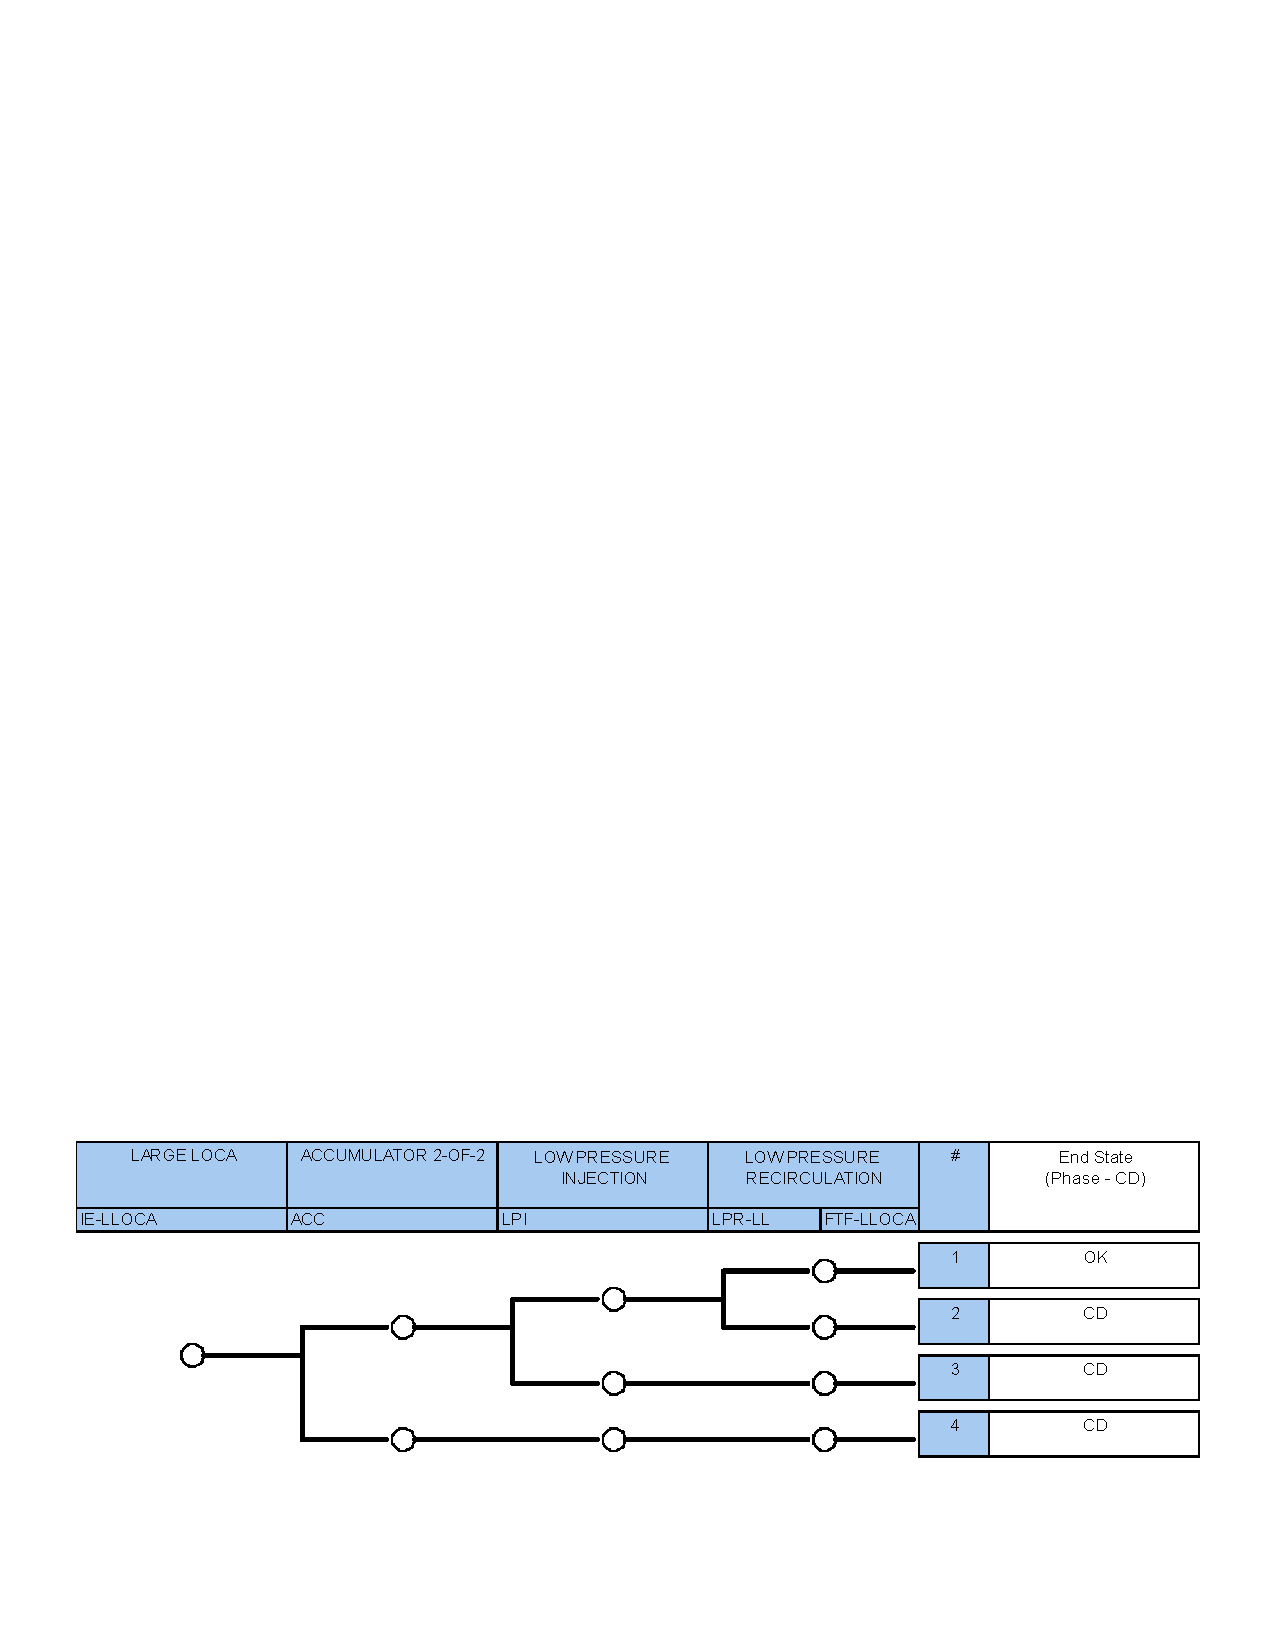
\includegraphics[scale=0.5]{ET_LLOCA.pdf}} 
    \caption{Large LOCA ET.}
    \label{fig:LLOCA_ET}
\end{figure}

In a dynamic PRA method, timing and sequencing of events are uniquely dictated by the system control logic
and by the set of stochastic parameters $\boldsymbol s$,i.e., the construction of the ET is replaced by coding 
the plant control logic (e.g., system activation points and activation rules).
In addition, acceptance criteria and success criteria are incorporated into the physics model of the code
Back to the large LOCA scenario, in a dynamic framework it would be modeled by:
\begin{itemize}
  \item employing a system simulator code (e.g., RELAP5-3D) 
  \item three stochastic parameters: 
        \begin{itemize}
          \item accumulator system: failure on demand (Bernoulli distribution)
          \item LPI system: failure to run (Exponential distribution)
          \item LPR system: failure to run (Exponential distribution)
        \end{itemize}
   \item the condition to end a code simulation run and its corresponding outcome:
        \begin{itemize}
          \item OK outcome: mission time (e.g., 24 hours)
          \item Fail outcome: max core temperature greater than 2200 F 
        \end{itemize}       
\end{itemize}

Note that a large discrepancies among classical and dynamic PRA methods can occur for large sequence of 
events coupled with system dynamics.
Assuming two events A and B occur in sequence and time of activation of each of them is a stochastic variable 
($t_A \sim pdf_A(t)$ and $t_B \sim pdf_B(t)$), the actual activation time $T_B$ of system B is a stochastic 
variable given by the sum of $t_A$ and $t_B$ ($T_B = t_A + t_B$). 
In a classical PRA framework, the distribution of $T_B$ (i.e., $pdf_{A+B}(t)$) can be 
determined by solving the convolution integral:   
\begin{equation}
  pdf_{A+B}(t) = \int_{-\infty}^{\infty} pdf_B(t-\tau) pdf_A(\tau) d\tau
  \label{eq:trajectory}
\end{equation}
This convolution integral get more complex when accident progression include a large number of events and 
system dynamics affect timing of events.




